\section{Appendix}\label{sec:Annexes}
%------------------------------------------------------------------------------------------------------------
%------------------------------------------------------------------------------------------------------------
%------------------------------------------------------------------------------------------------------------
%------------------------------------------------------------------------------------------------------------
\subsection*{Appendix A: Modes for rectangular duct}\label{sec:EigenvalueRect}
The duct geometry is:
\begin{figure}[H] \centering
    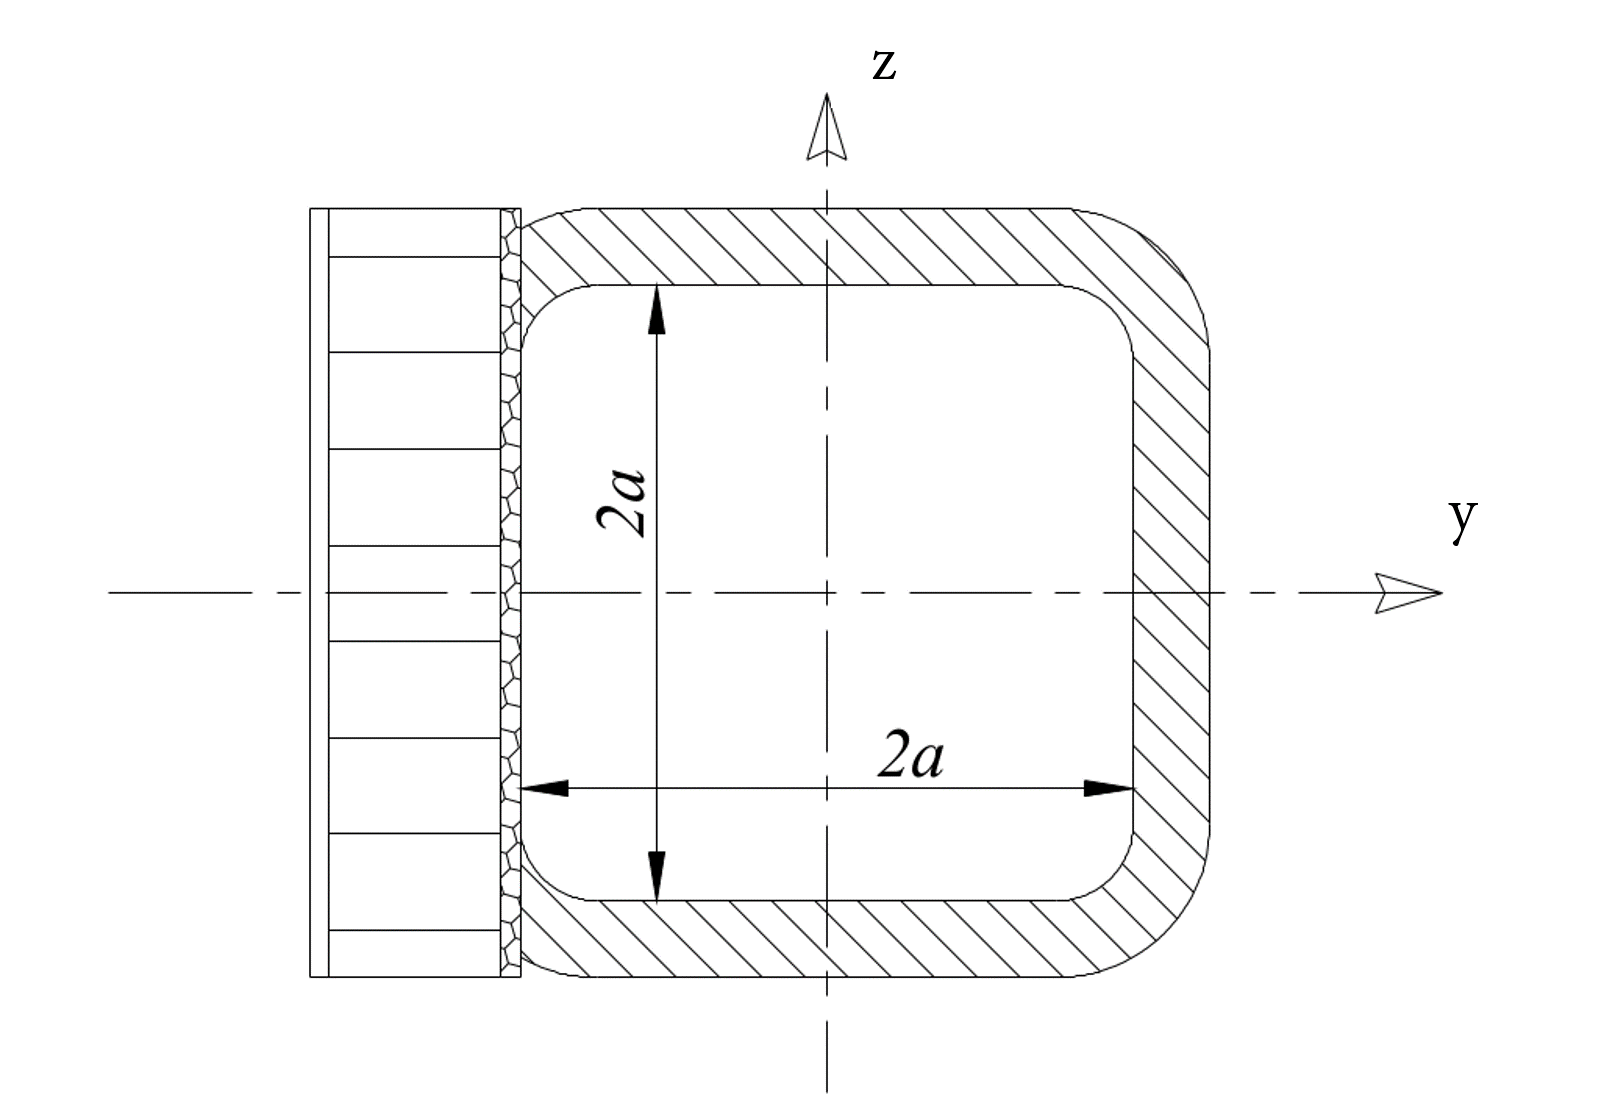
\includegraphics[scale=0.3]{Zhourectduct}
    \caption{Rectangular duct lined for y=-a}
\end{figure}
The Convective Helmholtz equation in the Cartesian coordinates:
\begin{equation}
    \Delta p +\Big[(w-ku_0)^2-k^2c_0^2\Big]p=0
\end{equation}
A resolution by separation of variables gives this decomposition:
\begin{equation}
    p(x,y,z,\omega)=\sum_{l=0}^\infty p_l^+ \Psi_{(m,n)}(x,y,z)+p_l^- \Psi_{(m,n)}(x,y,z)
\end{equation}
With:
\begin{equation}
    \Psi_{(m,n)}(x,y,z)=(A_me^{ik_{y,(m,n)}}+B_me^{-ik_{y,(m,n)}})(A_ne^{ik_{z,(m,n)}}+B_ne^{-ik_{z,(m,n)}})e^{-ik_{x,(m,n)}(M,\omega)x}
\end{equation}
%------------------------------------------------------------------------------------------------------------
%------------------------------------------------------------------------------------------------------------
\subsubsection*{Hard duct}\label{sec:EigenvalueHard}
Starting with the general form:
\begin{equation}
        \Psi(x,y,z)=(Ae^{ik_{y}y}+Be^{-ik_{y,l}y})(Ce^{ik_{z}z}+Dne^{-ik_{z}z})e^{-ik_{x}(M,\omega)x}
\end{equation}
The boundary conditions in the z direction are the hard wall conditions, the velocity is zero:  
\begin{equation}
    \frac{\partial\Psi}{\partial z} \Bigg|_{z=+a}=0
\end{equation}
Give the system:
\begin{equation}\label{eq:1}
    \left\{
    \begin{array}{ll}
    Ce^{-ik_za}-De^{ik_za}=0\\
        \\
    Ce^{ik_za}-De^{-ik_za}=0   
    \end{array}
    \right.
\end{equation}
In the matrix form: 
\begin{gather}
    \begin{bmatrix}
      e^{-ik_za} & -e^{ik_za} \\
      e^{ik_za} & -e^{-ik_za}
    \end{bmatrix}
    \begin{pmatrix}
       C\\
       D
    \end{pmatrix}
    =
    \begin{pmatrix}
      0\\
      0
    \end{pmatrix}
\end{gather}
The eigenvalue equation:
\begin{equation}
    -e^{-i2k_za}+e^{i2k_za}=0 \iff \sin(2ka)=0
\end{equation}
The wave number of order $n$:
\begin{equation}
    k_{z,n}=\frac{n\pi}{2a} \ ; \ n\in N
\end{equation}
Compute in the system Eq.\eqref{eq:1}
\begin{equation}
    \left\{
    \begin{array}{ll}
    C_ne^{-i\frac{n\pi}{2}}-D_ne^{i\frac{n\pi}{2}}=0\\
        \\
    C_ne^{i\frac{n\pi}{2}}-D_ne^{-i\frac{n\pi}{2}}=0   
    \end{array}
    \right.
\end{equation}
Thus:
\begin{equation}
    C_n(-i)^{n}-D_n(i)^{n}=0
\end{equation}
Two cases $n=2p$ or $n=2p+1$
\begin{equation}
    C_n=D_n \ \text{for} \ n=2p \ \text{and} \ C_n=-D_n\ \text{for} \ n=2p+1 
\end{equation}
Two solution for the shapes modes:
\begin{equation}
    \Psi_{n}(z)=2\cos(\frac{n\pi}{2a}z) \ \text{for} \ n=2p \ \text{and} \ \Psi_{n}(z)=2i\sin(\frac{n\pi}{2a}z)\ \text{for} \ n=2p+1 
\end{equation}
Finally for two opposite hard walls the shapes modes are: 
\begin{equation}
    \left\{
    \begin{array}{ll}
    \Psi_{n}(z)=2\cos(\frac{n\pi}{2a}z)\ \text{for} \ n=2p \\
        \\
    \Psi_{n}(z)=2i\sin(\frac{n\pi}{2a}z) \ \text{for} \ n=2p+1
    \end{array}
    \right.
\end{equation}
Note that only the modes below the cut-off frequency propagate. The higher mode are quickly attenuated. 
%------------------------------------------------------------------------------------------------------------
%------------------------------------------------------------------------------------------------------------
\subsubsection*{Lined walls}\label{sec:EigenvalueLined}
Starting with the general form:
\begin{equation}
        \Psi(x,y,z)=(Ae^{ik_{y}y}+Be^{-ik_{y,l}y})(Ce^{ik_{z}z}+Dne^{-ik_{z}z})e^{-ik_{x}(M,\omega)x}
\end{equation}
The boundary conditions in the y direction one lined wall and a hard wall, the velocity is respectively 0 and given by the Myers condition:
\begin{equation}
    \frac{\partial\Psi}{\partial y} \Big|_{y=+a}=0
\end{equation}
\begin{equation}
    \frac{\partial p}{\partial y}\Bigg|_{y=-a}=\frac{ik}{Z}(1-iM\frac{\partial}{\partial x})^2 p\Bigg|_{y=-a}
\end{equation}
Give the system:
\begin{equation}\label{eq:2}
    \left\{
    \begin{array}{ll}
    Ae^{ik_ya}-Be^{-ik_ya}=0\\
        \\
    Aik_ye^{-ik_ya}-Bik_ye^{ik_ya}=ikA(1-\frac{Mk_x}{k})[Ae^{-ik_ya}-Be^{ik_ya}]
    \end{array}
    \right.
\end{equation}
Using the wave dispersion equation:
\begin{equation}
   k_z^2+k_y^2=(k-Mk_x)^2 
\end{equation}
Using this relation in the Myers condition:
\begin{equation}
    \left\{
    \begin{array}{ll}
    Ae^{ik_ya}-Be^{-ik_ya}=0\\
        \\
    Ak_ye^{-ik_ya}-Bk_ye^{ik_ya}=\frac{A}{k}(k_z^2+k_y^2)^2[Ae^{-k_ya}-Be^{k_ya}]
    \end{array}
    \right.
\end{equation}\label{eq:3}
The matrix form: 
 \begin{gather}
    \begin{bmatrix}
     e^{ik_ya} & -e^{-ik_ya} \\
      \\
     k_ye^{-ik_ya}-\frac{A}{k}(k_z^2+k_y^2)^2[e^{-k_ya}] & -k_ye^{ik_ya}-\frac{A}{k}(k_z^2+k_y^2)^2[-e^{k_ya}]
    \end{bmatrix}
    \begin{pmatrix}
       A\\
       B
    \end{pmatrix}
    =
    \begin{pmatrix}
      0\\
      0
    \end{pmatrix}
 \end{gather}
The eigenvalue equation:
\begin{equation}
    -k_y(e^{i2k_ya}-e^{-i2k_ya})-(e^{2ik_ya}+e^{-2ik_ya})(\frac{A}{k}(k_z^2+k_y^2))=0
\end{equation}
The final eigenvalue equation:
\begin{equation} \label{eq:eigenlined}
    k_y\tan(2k_ya) -i(\frac{A}{k}(k_z^2+k_y^2))=0
\end{equation}
This equation has $m$ solution, called modes. Thus the wave number $k_{y,m}$ is the $m-th$ $k_r$ solution of the eigenvalue equation Eq.\eqref{eq:eigenlined}. 
The first line of the system Eq.\eqref{eq:3} gives an other condition for the amplitudes:
\begin{equation}
    A_me^{ik_{y,m}a}-B_me^{-ik_{y,m}a}=0 \iff  B_m=A_me^{i2k_{y,m}a}
\end{equation}
Finally for a lined wall opposite to a hard walls the shapes modes are: 
\begin{equation}
    \Psi_{m}(y)=e^{ik_{y,m}y}-e^{-ik_{y,m}(y-2a)}\ \text{with}\ k_{y,m} \ \text{solution of} \ Eq.\eqref{eq:eigenlined}
\end{equation}
Note than the relation:
\begin{equation}
   \frac{\frac{\partial\Psi_{l}}{\partial y}|_{y=-a}}{p|_{y=-a}}=k_y\tan(2k_ya)
\end{equation}
And compute in the Myers boundary conditions gives directly the impedance:
\begin{equation}\label{eq:Impedance}
   Z=\frac{i(k-Mk_x)^2}{k\ k_z\tan(2ak_x)}
\end{equation}
%------------------------------------------------------------------------------------------------------------
%------------------------------------------------------------------------------------------------------------
%------------------------------------------------------------------------------------------------------------
%------------------------------------------------------------------------------------------------------------
\subsection*{Appendix B: Cremer optimum resolution with matlab}\label{sec:AppendixB}
The circular resolution is very similar to the annular resolution.
The least attenuated mode is the $(m,n)$ and the radial wave number is $k_r=k_{r,(m,n)}$. A function $F(k_r)$ is defined as the derivative of the eigenvalue equation. The function "vpsole" solve $F=0$ using a starting point called "initial guess". \\
To preliminary find the "initial guess point", $1/F(k_r)$ is ploted in the complex plan: 
\begin{figure}[H] \centering
    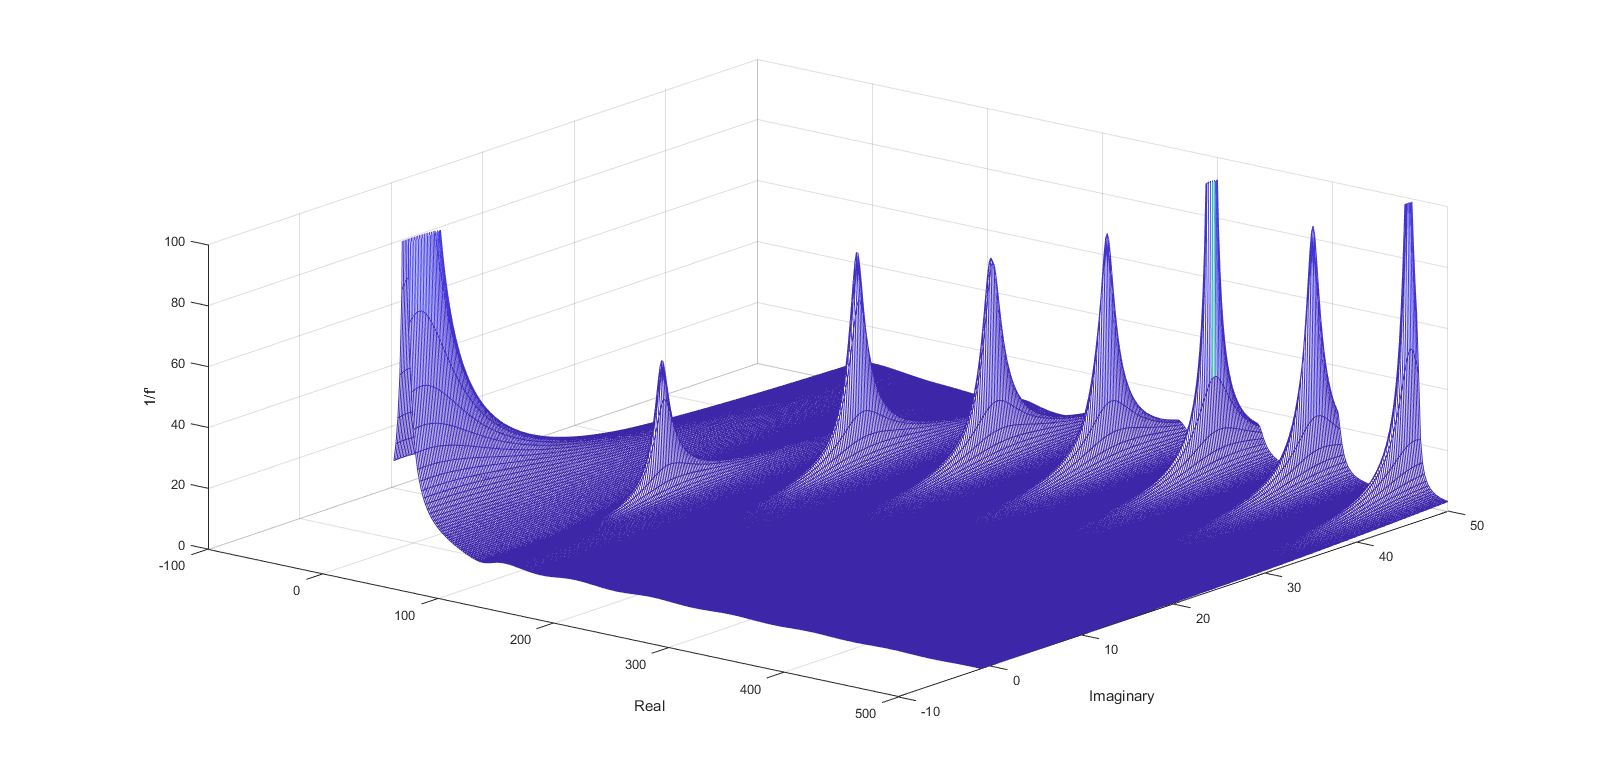
\includegraphics[scale=0.3]{1_Fctannulaire13D}
    \caption{$1/F(k_r)$ in the complex plan}
\end{figure}
Every peak correspond to a root of $F(k_r)$ and the approximate coordinates are used in the "vpsovle" as initial guess.\\
The first $n$ solutions are represented in the graph:
\begin{figure}[H] \centering
    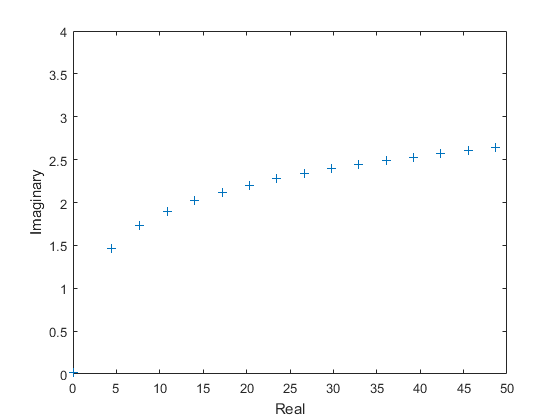
\includegraphics[scale=0.7]{Solutionscyl2D}
    \caption{$k_{r,(1,n)}$ solution of $F=0$ for the circular case}
\end{figure}
The $n$ non zero is the optimum radial wave number $k_{r,(m,n)}$ 
%------------------------------------------------------------------------------------------------------------
%------------------------------------------------------------------------------------------------------------
%------------------------------------------------------------------------------------------------------------
%------------------------------------------------------------------------------------------------------------
\subsection*{Appendix C: Mean flow measurement}\label{sec:AppendixC}
The Pitot tube measures the dynamic $p_t$ pressure thanks to a manometer. The atmospheric pressure is called $P_s$.
Two models exist:
\begin{itemize}
    \item Incompressible fluid
        \begin{equation}
        u = \sqrt{\frac{2(p_t-p_s)}{\rho}}         
        \end{equation}
        \item Compressible fluid
        \begin{equation}
        \frac{p_t}{p_s} = \Big(1+\frac{\gamma-1}{2}  M^2\Big)^{\frac{\gamma}{\gamma-1}}    
        \end{equation}
\end{itemize}
The two models are drawn in a graphic:
\begin{figure}[H] \centering
    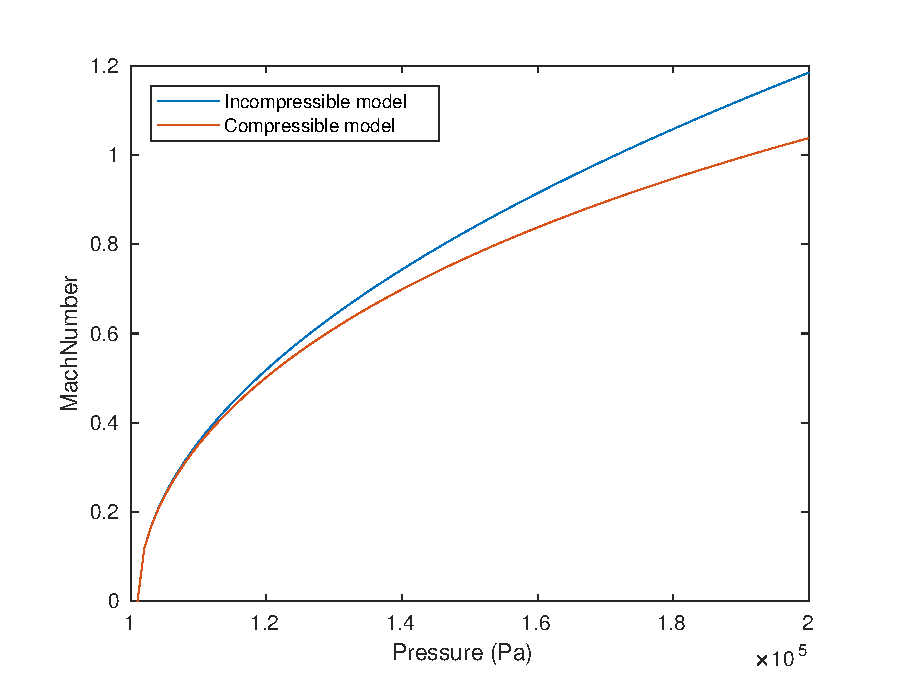
\includegraphics[scale=0.7]{MachModels}
    \caption{Two different models for Pitot tube}
\end{figure}
\noindent For mach number belove $0.2$ both models give approximately the same value.\\
However, the pressure is measured in the middle of the section and get the maximal velocity. Indeed the profil of the velocity across the section is not uniform as showed the following graphic:
\begin{figure}[H] \centering
    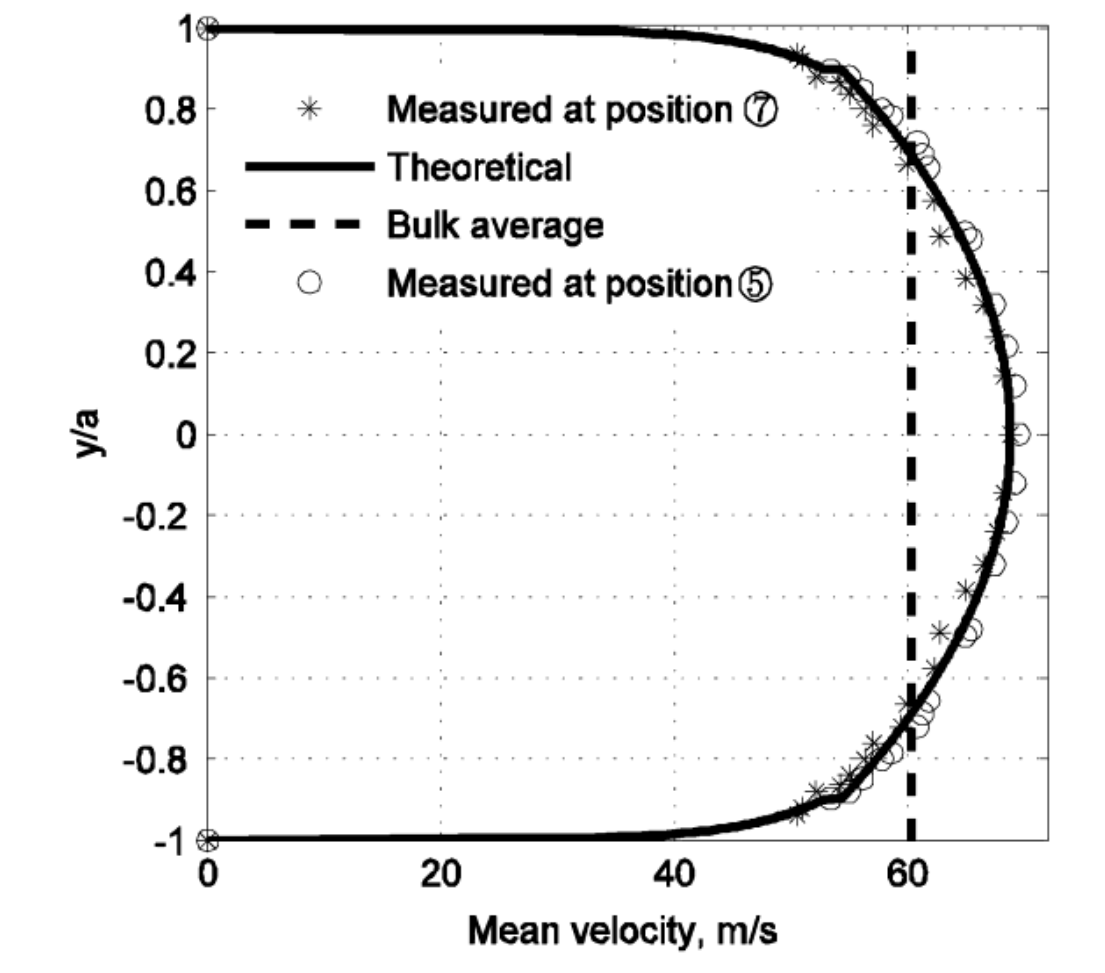
\includegraphics[scale=0.2]{FlowProfil}
    \caption{Flow profile across a section \cite{Zhou_thesis}}
\end{figure}
\noindent A correction coefficient between the mean mach number and the maximum mach number is applied. It was determined with a linear regression based on experimental values \cite{Zhou_thesis}.
\begin{figure}[H] \centering
    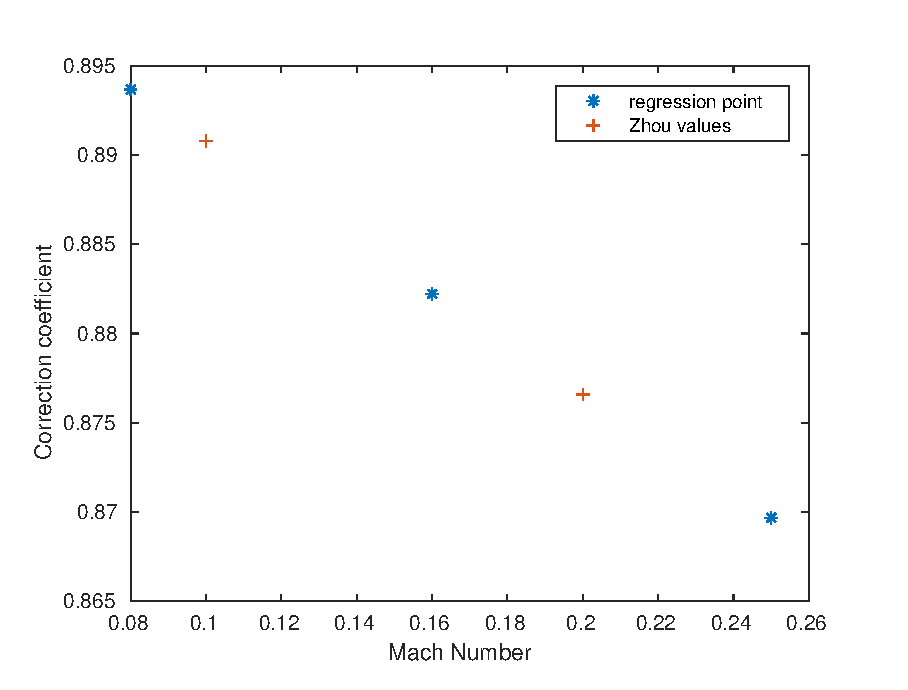
\includegraphics[scale=0.7]{LinearRegretion}
    \caption{Linear regression}
\end{figure}
The target mach numbers used in this report were 0.08 and 0.16 and are the mean mach number value.